\documentclass{standalone}
\usepackage{tikz}

\begin{document}
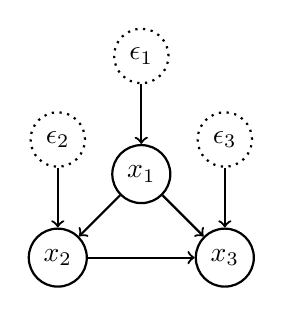
\begin{tikzpicture}[node distance={15mm}, thick, main/.style = {draw, circle}]
    \node[main] (1) {$x_1$};
    \node[main] (2) [below left of=1] {$x_2$};
    \node[main] (3) [below right of=1] {$x_3$};
    \node[main, dotted] (4) [above of=1] {$\epsilon_1$};
    \node[main, dotted] (5) [above of=2] {$\epsilon_2$};
    \node[main, dotted] (6) [above of=3] {$\epsilon_3$};

    \draw[->] (1) -- (2);
    \draw[->] (1) -- (3);
    \draw[->] (2) -- (3);
    \draw[->] (4) -- (1);
    \draw[->] (5) -- (2);
    \draw[->] (6) -- (3);

    \end{tikzpicture}
\end{document}
